% Created by tikzDevice version 0.12.3.1 on 2022-05-02 11:32:24
% !TEX encoding = UTF-8 Unicode
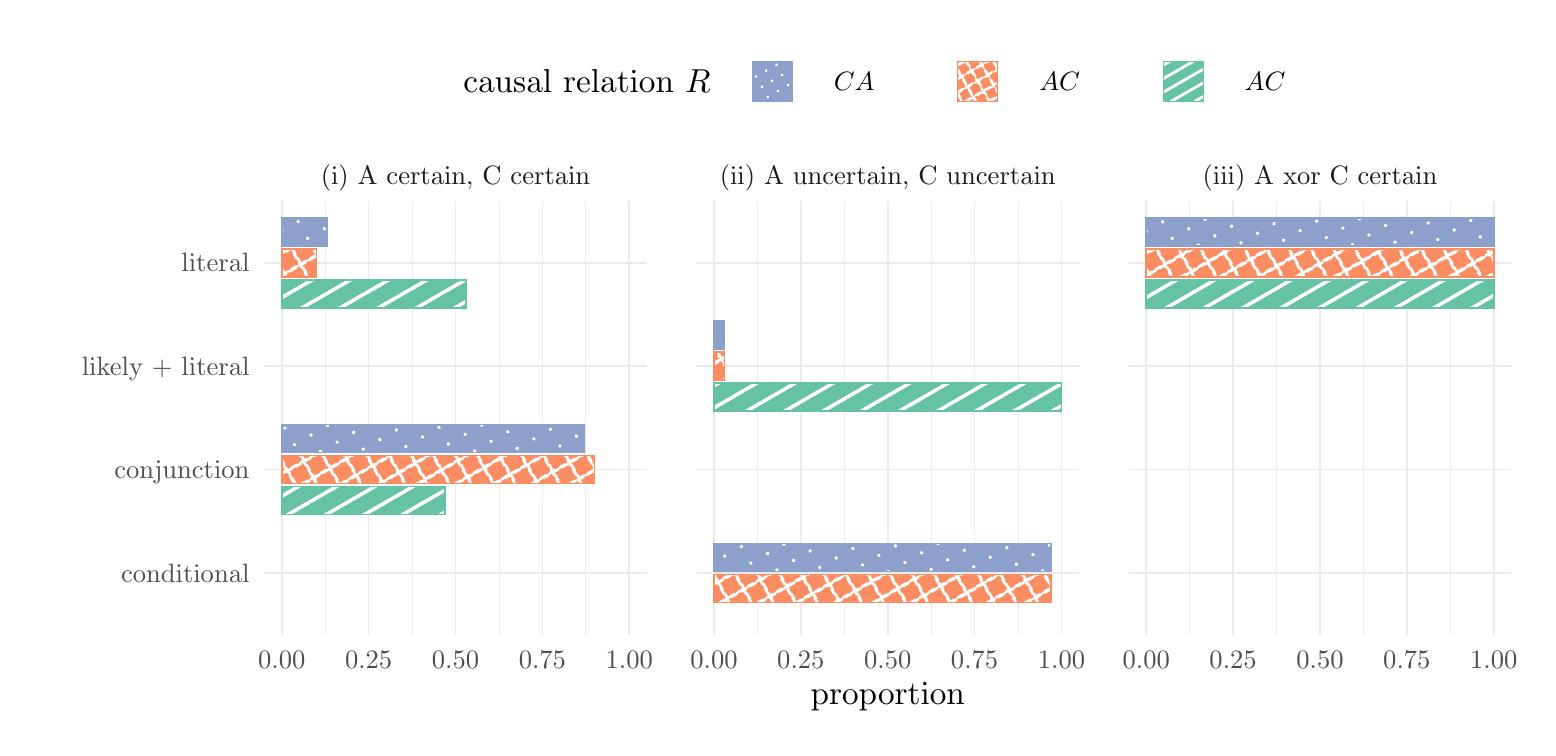
\begin{tikzpicture}[x=1pt,y=1pt]
\definecolor{fillColor}{RGB}{255,255,255}
\path[use as bounding box,fill=fillColor,fill opacity=0.00] (0,0) rectangle (542.02,252.94);
\begin{scope}
\path[clip] ( 85.54, 33.48) rectangle (223.66,190.41);
\definecolor{drawColor}{gray}{0.92}

\path[draw=drawColor,line width= 0.3pt,line join=round] (107.52, 33.48) --
	(107.52,190.41);

\path[draw=drawColor,line width= 0.3pt,line join=round] (138.91, 33.48) --
	(138.91,190.41);

\path[draw=drawColor,line width= 0.3pt,line join=round] (170.30, 33.48) --
	(170.30,190.41);

\path[draw=drawColor,line width= 0.3pt,line join=round] (201.69, 33.48) --
	(201.69,190.41);

\path[draw=drawColor,line width= 0.6pt,line join=round] ( 85.54, 55.90) --
	(223.66, 55.90);

\path[draw=drawColor,line width= 0.6pt,line join=round] ( 85.54, 93.26) --
	(223.66, 93.26);

\path[draw=drawColor,line width= 0.6pt,line join=round] ( 85.54,130.63) --
	(223.66,130.63);

\path[draw=drawColor,line width= 0.6pt,line join=round] ( 85.54,167.99) --
	(223.66,167.99);

\path[draw=drawColor,line width= 0.6pt,line join=round] ( 91.82, 33.48) --
	( 91.82,190.41);

\path[draw=drawColor,line width= 0.6pt,line join=round] (123.21, 33.48) --
	(123.21,190.41);

\path[draw=drawColor,line width= 0.6pt,line join=round] (154.60, 33.48) --
	(154.60,190.41);

\path[draw=drawColor,line width= 0.6pt,line join=round] (185.99, 33.48) --
	(185.99,190.41);

\path[draw=drawColor,line width= 0.6pt,line join=round] (217.38, 33.48) --
	(217.38,190.41);
\definecolor{fillColor}{RGB}{102,194,165}

\path[fill=fillColor] ( 91.82, 77.01) rectangle (150.83, 87.10);
\definecolor{fillColor}{RGB}{252,141,98}

\path[fill=fillColor] ( 91.82, 88.22) rectangle (204.82, 98.31);
\definecolor{fillColor}{RGB}{141,160,203}

\path[fill=fillColor] ( 91.82, 99.43) rectangle (201.06,109.52);
\definecolor{fillColor}{RGB}{102,194,165}

\path[fill=fillColor] ( 91.82,151.74) rectangle (158.37,161.83);
\definecolor{fillColor}{RGB}{252,141,98}

\path[fill=fillColor] ( 91.82,162.95) rectangle (104.38,173.04);
\definecolor{fillColor}{RGB}{141,160,203}

\path[fill=fillColor] ( 91.82,174.16) rectangle (108.14,184.25);
\definecolor{drawColor}{RGB}{255,255,255}
\definecolor{fillColor}{RGB}{255,255,255}

\path[draw=drawColor,line width= 0.6pt,line join=round,line cap=rect,fill=fillColor] (148.64, 77.01) --
	(150.83, 78.27) --
	(150.83, 77.47) --
	(150.02, 77.01) --
	(148.64, 77.01) --
	cycle;

\path[draw=drawColor,line width= 0.6pt,line join=round,line cap=rect,fill=fillColor] (134.83, 77.01) --
	(150.83, 86.25) --
	(150.83, 85.45) --
	(136.21, 77.01) --
	(134.83, 77.01) --
	cycle;

\path[draw=drawColor,line width= 0.6pt,line join=round,line cap=rect,fill=fillColor] (121.02, 77.01) --
	(138.49, 87.10) --
	(139.88, 87.10) --
	(122.40, 77.01) --
	(121.02, 77.01) --
	cycle;

\path[draw=drawColor,line width= 0.6pt,line join=round,line cap=rect,fill=fillColor] (107.21, 77.01) --
	(124.68, 87.10) --
	(126.06, 87.10) --
	(108.59, 77.01) --
	(107.21, 77.01) --
	cycle;

\path[draw=drawColor,line width= 0.6pt,line join=round,line cap=rect,fill=fillColor] ( 93.40, 77.01) --
	(110.87, 87.10) --
	(112.25, 87.10) --
	( 94.78, 77.01) --
	( 93.40, 77.01) --
	cycle;

\path[draw=drawColor,line width= 0.6pt,line join=round,line cap=rect,fill=fillColor] ( 91.82, 84.07) --
	( 97.06, 87.10) --
	( 98.44, 87.10) --
	( 91.82, 83.27) --
	( 91.82, 84.07) --
	cycle;

\path[draw=drawColor,line width= 0.6pt,dash pattern=on 2pt off 2pt ,line join=round,line cap=rect,fill=fillColor] (195.68, 88.22) --
	(204.82, 93.49) --
	(204.82, 92.70) --
	(197.06, 88.22) --
	(195.68, 88.22) --
	cycle;

\path[draw=drawColor,line width= 0.6pt,dash pattern=on 2pt off 2pt ,line join=round,line cap=rect,fill=fillColor] (181.87, 88.22) --
	(199.35, 98.31) --
	(200.73, 98.31) --
	(183.25, 88.22) --
	(181.87, 88.22) --
	cycle;

\path[draw=drawColor,line width= 0.6pt,dash pattern=on 2pt off 2pt ,line join=round,line cap=rect,fill=fillColor] (168.06, 88.22) --
	(185.53, 98.31) --
	(186.91, 98.31) --
	(169.44, 88.22) --
	(168.06, 88.22) --
	cycle;

\path[draw=drawColor,line width= 0.6pt,dash pattern=on 2pt off 2pt ,line join=round,line cap=rect,fill=fillColor] (154.25, 88.22) --
	(171.72, 98.31) --
	(173.10, 98.31) --
	(155.63, 88.22) --
	(154.25, 88.22) --
	cycle;

\path[draw=drawColor,line width= 0.6pt,dash pattern=on 2pt off 2pt ,line join=round,line cap=rect,fill=fillColor] (140.44, 88.22) --
	(157.91, 98.31) --
	(159.29, 98.31) --
	(141.82, 88.22) --
	(140.44, 88.22) --
	cycle;

\path[draw=drawColor,line width= 0.6pt,dash pattern=on 2pt off 2pt ,line join=round,line cap=rect,fill=fillColor] (126.62, 88.22) --
	(144.10, 98.31) --
	(145.48, 98.31) --
	(128.01, 88.22) --
	(126.62, 88.22) --
	cycle;

\path[draw=drawColor,line width= 0.6pt,dash pattern=on 2pt off 2pt ,line join=round,line cap=rect,fill=fillColor] (112.81, 88.22) --
	(130.29, 98.31) --
	(131.67, 98.31) --
	(114.19, 88.22) --
	(112.81, 88.22) --
	cycle;

\path[draw=drawColor,line width= 0.6pt,dash pattern=on 2pt off 2pt ,line join=round,line cap=rect,fill=fillColor] ( 99.00, 88.22) --
	(116.48, 98.31) --
	(117.86, 98.31) --
	(100.38, 88.22) --
	( 99.00, 88.22) --
	cycle;

\path[draw=drawColor,line width= 0.6pt,dash pattern=on 2pt off 2pt ,line join=round,line cap=rect,fill=fillColor] ( 91.82, 92.05) --
	(102.66, 98.31) --
	(104.05, 98.31) --
	( 91.82, 91.25) --
	( 91.82, 92.05) --
	cycle;

\path[draw=drawColor,line width= 0.6pt,dash pattern=on 2pt off 2pt ,line join=round,line cap=rect,fill=fillColor] ( 91.82, 97.07) --
	( 96.93, 88.22) --
	( 96.13, 88.22) --
	( 91.82, 95.69) --
	( 91.82, 97.07) --
	cycle;

\path[draw=drawColor,line width= 0.6pt,dash pattern=on 2pt off 2pt ,line join=round,line cap=rect,fill=fillColor] ( 99.08, 98.31) --
	(104.91, 88.22) --
	(104.11, 88.22) --
	( 98.28, 98.31) --
	( 99.08, 98.31) --
	cycle;

\path[draw=drawColor,line width= 0.6pt,dash pattern=on 2pt off 2pt ,line join=round,line cap=rect,fill=fillColor] (107.06, 98.31) --
	(112.88, 88.22) --
	(112.08, 88.22) --
	(106.26, 98.31) --
	(107.06, 98.31) --
	cycle;

\path[draw=drawColor,line width= 0.6pt,dash pattern=on 2pt off 2pt ,line join=round,line cap=rect,fill=fillColor] (115.03, 98.31) --
	(120.85, 88.22) --
	(120.06, 88.22) --
	(114.23, 98.31) --
	(115.03, 98.31) --
	cycle;

\path[draw=drawColor,line width= 0.6pt,dash pattern=on 2pt off 2pt ,line join=round,line cap=rect,fill=fillColor] (123.00, 98.31) --
	(128.83, 88.22) --
	(128.03, 88.22) --
	(122.21, 98.31) --
	(123.00, 98.31) --
	cycle;

\path[draw=drawColor,line width= 0.6pt,dash pattern=on 2pt off 2pt ,line join=round,line cap=rect,fill=fillColor] (130.98, 98.31) --
	(136.80, 88.22) --
	(136.00, 88.22) --
	(130.18, 98.31) --
	(130.98, 98.31) --
	cycle;

\path[draw=drawColor,line width= 0.6pt,dash pattern=on 2pt off 2pt ,line join=round,line cap=rect,fill=fillColor] (138.95, 98.31) --
	(144.78, 88.22) --
	(143.98, 88.22) --
	(138.15, 98.31) --
	(138.95, 98.31) --
	cycle;

\path[draw=drawColor,line width= 0.6pt,dash pattern=on 2pt off 2pt ,line join=round,line cap=rect,fill=fillColor] (146.93, 98.31) --
	(152.75, 88.22) --
	(151.95, 88.22) --
	(146.13, 98.31) --
	(146.93, 98.31) --
	cycle;

\path[draw=drawColor,line width= 0.6pt,dash pattern=on 2pt off 2pt ,line join=round,line cap=rect,fill=fillColor] (154.90, 98.31) --
	(160.72, 88.22) --
	(159.93, 88.22) --
	(154.10, 98.31) --
	(154.90, 98.31) --
	cycle;

\path[draw=drawColor,line width= 0.6pt,dash pattern=on 2pt off 2pt ,line join=round,line cap=rect,fill=fillColor] (162.87, 98.31) --
	(168.70, 88.22) --
	(167.90, 88.22) --
	(162.08, 98.31) --
	(162.87, 98.31) --
	cycle;

\path[draw=drawColor,line width= 0.6pt,dash pattern=on 2pt off 2pt ,line join=round,line cap=rect,fill=fillColor] (170.85, 98.31) --
	(176.67, 88.22) --
	(175.88, 88.22) --
	(170.05, 98.31) --
	(170.85, 98.31) --
	cycle;

\path[draw=drawColor,line width= 0.6pt,dash pattern=on 2pt off 2pt ,line join=round,line cap=rect,fill=fillColor] (178.82, 98.31) --
	(184.65, 88.22) --
	(183.85, 88.22) --
	(178.02, 98.31) --
	(178.82, 98.31) --
	cycle;

\path[draw=drawColor,line width= 0.6pt,dash pattern=on 2pt off 2pt ,line join=round,line cap=rect,fill=fillColor] (186.80, 98.31) --
	(192.62, 88.22) --
	(191.82, 88.22) --
	(186.00, 98.31) --
	(186.80, 98.31) --
	cycle;

\path[draw=drawColor,line width= 0.6pt,dash pattern=on 2pt off 2pt ,line join=round,line cap=rect,fill=fillColor] (194.77, 98.31) --
	(200.60, 88.22) --
	(199.80, 88.22) --
	(193.97, 98.31) --
	(194.77, 98.31) --
	cycle;

\path[draw=drawColor,line width= 0.6pt,dash pattern=on 2pt off 2pt ,line join=round,line cap=rect,fill=fillColor] (202.74, 98.31) --
	(204.82, 94.70) --
	(204.82, 93.32) --
	(201.95, 98.31) --
	(202.74, 98.31) --
	cycle;

\path[draw=drawColor,line width= 0.6pt,dash pattern=on 4pt off 2pt ,line join=round,line cap=round,fill=fillColor] ( 92.94,108.24) circle (  0.35);

\path[draw=drawColor,line width= 0.6pt,dash pattern=on 4pt off 2pt ,line join=round,line cap=round,fill=fillColor] ( 96.40,102.26) circle (  0.35);

\path[draw=drawColor,line width= 0.6pt,dash pattern=on 4pt off 2pt ,line join=round,line cap=round,fill=fillColor] (102.38,105.72) circle (  0.35);

\path[draw=drawColor,line width= 0.6pt,dash pattern=on 4pt off 2pt ,line join=round,line cap=round,fill=fillColor] (108.36,109.17) circle (  0.35);

\path[draw=drawColor,line width= 0.6pt,dash pattern=on 4pt off 2pt ,line join=round,line cap=round,fill=fillColor] (111.81,103.19) circle (  0.35);

\path[draw=drawColor,line width= 0.6pt,dash pattern=on 4pt off 2pt ,line join=round,line cap=round,fill=fillColor] (117.79,106.64) circle (  0.35);

\path[draw=drawColor,line width= 0.6pt,dash pattern=on 4pt off 2pt ,line join=round,line cap=round,fill=fillColor] (121.25,100.66) circle (  0.35);

\path[draw=drawColor,line width= 0.6pt,dash pattern=on 4pt off 2pt ,line join=round,line cap=round,fill=fillColor] (127.23,104.11) circle (  0.35);

\path[draw=drawColor,line width= 0.6pt,dash pattern=on 4pt off 2pt ,line join=round,line cap=round,fill=fillColor] (133.21,107.57) circle (  0.35);

\path[draw=drawColor,line width= 0.6pt,dash pattern=on 4pt off 2pt ,line join=round,line cap=round,fill=fillColor] (136.66,101.59) circle (  0.35);

\path[draw=drawColor,line width= 0.6pt,dash pattern=on 4pt off 2pt ,line join=round,line cap=round,fill=fillColor] (142.64,105.04) circle (  0.35);

\path[draw=drawColor,line width= 0.6pt,dash pattern=on 4pt off 2pt ,line join=round,line cap=round,fill=fillColor] (148.62,108.49) circle (  0.35);

\path[draw=drawColor,line width= 0.6pt,dash pattern=on 4pt off 2pt ,line join=round,line cap=round,fill=fillColor] (152.07,102.51) circle (  0.35);

\path[draw=drawColor,line width= 0.6pt,dash pattern=on 4pt off 2pt ,line join=round,line cap=round,fill=fillColor] (158.05,105.96) circle (  0.35);

\path[draw=drawColor,line width= 0.6pt,dash pattern=on 4pt off 2pt ,line join=round,line cap=round,fill=fillColor] (161.51, 99.98) circle (  0.35);

\path[draw=drawColor,line width= 0.6pt,dash pattern=on 4pt off 2pt ,line join=round,line cap=round,fill=fillColor] (167.49,103.44) circle (  0.35);

\path[draw=drawColor,line width= 0.6pt,dash pattern=on 4pt off 2pt ,line join=round,line cap=round,fill=fillColor] (173.47,106.89) circle (  0.35);

\path[draw=drawColor,line width= 0.6pt,dash pattern=on 4pt off 2pt ,line join=round,line cap=round,fill=fillColor] (176.92,100.91) circle (  0.35);

\path[draw=drawColor,line width= 0.6pt,dash pattern=on 4pt off 2pt ,line join=round,line cap=round,fill=fillColor] (182.90,104.36) circle (  0.35);

\path[draw=drawColor,line width= 0.6pt,dash pattern=on 4pt off 2pt ,line join=round,line cap=round,fill=fillColor] (188.88,107.81) circle (  0.35);

\path[draw=drawColor,line width= 0.6pt,dash pattern=on 4pt off 2pt ,line join=round,line cap=round,fill=fillColor] (192.33,101.83) circle (  0.35);

\path[draw=drawColor,line width= 0.6pt,dash pattern=on 4pt off 2pt ,line join=round,line cap=round,fill=fillColor] (198.32,105.29) circle (  0.35);

\path[draw=drawColor,line width= 0.6pt,dash pattern=on 4pt off 2pt ,line join=round,line cap=round,fill=fillColor] (105.68, 99.43) --
	(105.67, 99.43) --
	(105.65, 99.44) --
	(105.63, 99.45) --
	(105.62, 99.46) --
	(105.60, 99.48) --
	(105.58, 99.49) --
	(105.57, 99.51) --
	(105.56, 99.53) --
	(105.54, 99.54) --
	(105.53, 99.56) --
	(105.52, 99.58) --
	(105.51, 99.60) --
	(105.50, 99.62) --
	(105.50, 99.64) --
	(105.49, 99.66) --
	(105.49, 99.68) --
	(105.49, 99.71) --
	(105.49, 99.73) --
	(105.49, 99.75) --
	(105.49, 99.77) --
	(105.49, 99.79) --
	(105.49, 99.81) --
	(105.50, 99.83) --
	(105.51, 99.86) --
	(105.52, 99.88) --
	(105.52, 99.90) --
	(105.54, 99.91) --
	(105.55, 99.93) --
	(105.56, 99.95) --
	(105.57, 99.97) --
	(105.59, 99.98) --
	(105.61,100.00) --
	(105.62,100.01) --
	(105.64,100.02) --
	(105.66,100.03) --
	(105.68,100.04) --
	(105.70,100.05) --
	(105.72,100.06) --
	(105.74,100.07) --
	(105.76,100.07) --
	(105.78,100.08) --
	(105.80,100.08) --
	(105.82,100.08) --
	(105.85,100.08) --
	(105.87,100.08) --
	(105.89,100.08) --
	(105.91,100.07) --
	(105.93,100.07) --
	(105.95,100.06) --
	(105.97,100.05) --
	(105.99,100.04) --
	(106.01,100.03) --
	(106.03,100.02) --
	(106.05,100.01) --
	(106.06, 99.99) --
	(106.08, 99.98) --
	(106.09, 99.96) --
	(106.11, 99.94) --
	(106.12, 99.93) --
	(106.13, 99.91) --
	(106.14, 99.89) --
	(106.15, 99.87) --
	(106.16, 99.85) --
	(106.16, 99.83) --
	(106.17, 99.81) --
	(106.17, 99.79) --
	(106.18, 99.76) --
	(106.18, 99.74) --
	(106.18, 99.72) --
	(106.17, 99.70) --
	(106.17, 99.68) --
	(106.17, 99.66) --
	(106.16, 99.64) --
	(106.15, 99.61) --
	(106.15, 99.59) --
	(106.14, 99.58) --
	(106.13, 99.56) --
	(106.11, 99.54) --
	(106.10, 99.52) --
	(106.09, 99.50) --
	(106.07, 99.49) --
	(106.06, 99.47) --
	(106.04, 99.46) --
	(106.02, 99.45) --
	(106.00, 99.44) --
	(105.99, 99.43) --
	(105.68, 99.43) --
	cycle;

\path[draw=drawColor,line width= 0.6pt,dash pattern=on 4pt off 2pt ,line join=round,line cap=round,fill=fillColor] (164.36,109.52) --
	(164.37,109.51) --
	(164.37,109.49) --
	(164.38,109.47) --
	(164.38,109.45) --
	(164.38,109.42) --
	(164.38,109.40) --
	(164.38,109.38) --
	(164.37,109.36) --
	(164.37,109.34) --
	(164.36,109.32) --
	(164.36,109.30) --
	(164.35,109.28) --
	(164.34,109.26) --
	(164.33,109.24) --
	(164.32,109.22) --
	(164.30,109.20) --
	(164.29,109.19) --
	(164.28,109.17) --
	(164.26,109.16) --
	(164.24,109.14) --
	(164.23,109.13) --
	(164.21,109.12) --
	(164.19,109.11) --
	(164.17,109.10) --
	(164.15,109.09) --
	(164.13,109.08) --
	(164.11,109.08) --
	(164.08,109.07) --
	(164.06,109.07) --
	(164.04,109.07) --
	(164.02,109.07) --
	(164.00,109.07) --
	(163.98,109.08) --
	(163.96,109.08) --
	(163.93,109.09) --
	(163.91,109.09) --
	(163.89,109.10) --
	(163.87,109.11) --
	(163.86,109.12) --
	(163.84,109.13) --
	(163.82,109.15) --
	(163.80,109.16) --
	(163.79,109.17) --
	(163.77,109.19) --
	(163.76,109.21) --
	(163.75,109.23) --
	(163.74,109.24) --
	(163.73,109.26) --
	(163.72,109.28) --
	(163.71,109.30) --
	(163.70,109.32) --
	(163.70,109.34) --
	(163.69,109.37) --
	(163.69,109.39) --
	(163.69,109.41) --
	(163.69,109.43) --
	(163.69,109.45) --
	(163.69,109.47) --
	(163.70,109.50) --
	(163.70,109.52) --
	(164.36,109.52) --
	cycle;

\path[draw=drawColor,line width= 0.6pt,line join=round,line cap=rect,fill=fillColor] (153.78,151.74) --
	(158.37,154.39) --
	(158.37,153.59) --
	(155.16,151.74) --
	(153.78,151.74) --
	cycle;

\path[draw=drawColor,line width= 0.6pt,line join=round,line cap=rect,fill=fillColor] (139.97,151.74) --
	(157.44,161.83) --
	(158.37,161.83) --
	(158.37,161.56) --
	(141.35,151.74) --
	(139.97,151.74) --
	cycle;

\path[draw=drawColor,line width= 0.6pt,line join=round,line cap=rect,fill=fillColor] (126.16,151.74) --
	(143.63,161.83) --
	(145.01,161.83) --
	(127.54,151.74) --
	(126.16,151.74) --
	cycle;

\path[draw=drawColor,line width= 0.6pt,line join=round,line cap=rect,fill=fillColor] (112.34,151.74) --
	(129.82,161.83) --
	(131.20,161.83) --
	(113.73,151.74) --
	(112.34,151.74) --
	cycle;

\path[draw=drawColor,line width= 0.6pt,line join=round,line cap=rect,fill=fillColor] ( 98.53,151.74) --
	(116.01,161.83) --
	(117.39,161.83) --
	( 99.91,151.74) --
	( 98.53,151.74) --
	cycle;

\path[draw=drawColor,line width= 0.6pt,line join=round,line cap=rect,fill=fillColor] ( 91.82,155.84) --
	(102.20,161.83) --
	(103.58,161.83) --
	( 91.82,155.04) --
	( 91.82,155.84) --
	cycle;

\path[draw=drawColor,line width= 0.6pt,dash pattern=on 2pt off 2pt ,line join=round,line cap=rect,fill=fillColor] (104.14,162.95) --
	(104.38,163.09) --
	(104.38,162.95) --
	(104.14,162.95) --
	cycle;

\path[draw=drawColor,line width= 0.6pt,dash pattern=on 2pt off 2pt ,line join=round,line cap=rect,fill=fillColor] ( 91.82,163.81) --
	(104.38,171.06) --
	(104.38,170.26) --
	( 91.82,163.01) --
	( 91.82,163.81) --
	cycle;

\path[draw=drawColor,line width= 0.6pt,dash pattern=on 2pt off 2pt ,line join=round,line cap=rect,fill=fillColor] ( 91.82,171.79) --
	( 93.99,173.04) --
	( 95.37,173.04) --
	( 91.82,170.99) --
	( 91.82,171.79) --
	cycle;

\path[draw=drawColor,line width= 0.6pt,dash pattern=on 2pt off 2pt ,line join=round,line cap=rect,fill=fillColor] ( 91.82,166.13) --
	( 93.66,162.95) --
	( 92.86,162.95) --
	( 91.82,164.75) --
	( 91.82,166.13) --
	cycle;

\path[draw=drawColor,line width= 0.6pt,dash pattern=on 2pt off 2pt ,line join=round,line cap=rect,fill=fillColor] ( 95.80,173.04) --
	(101.63,162.95) --
	(100.83,162.95) --
	( 95.01,173.04) --
	( 95.80,173.04) --
	cycle;

\path[draw=drawColor,line width= 0.6pt,dash pattern=on 2pt off 2pt ,line join=round,line cap=rect,fill=fillColor] (103.78,173.04) --
	(104.38,172.00) --
	(104.38,170.62) --
	(102.98,173.04) --
	(103.78,173.04) --
	cycle;

\path[draw=drawColor,line width= 0.6pt,dash pattern=on 4pt off 2pt ,line join=round,line cap=round,fill=fillColor] ( 97.75,182.79) circle (  0.35);

\path[draw=drawColor,line width= 0.6pt,dash pattern=on 4pt off 2pt ,line join=round,line cap=round,fill=fillColor] (101.20,176.81) circle (  0.35);

\path[draw=drawColor,line width= 0.6pt,dash pattern=on 4pt off 2pt ,line join=round,line cap=round,fill=fillColor] (107.19,180.26) circle (  0.35);

\path[draw=drawColor,line width= 0.6pt,dash pattern=on 4pt off 2pt ,line join=round,line cap=round,fill=fillColor] ( 91.82,179.67) --
	( 91.83,179.67) --
	( 91.85,179.67) --
	( 91.87,179.66) --
	( 91.89,179.66) --
	( 91.91,179.65) --
	( 91.93,179.64) --
	( 91.95,179.63) --
	( 91.97,179.62) --
	( 91.99,179.60) --
	( 92.00,179.59) --
	( 92.02,179.57) --
	( 92.03,179.56) --
	( 92.05,179.54) --
	( 92.06,179.52) --
	( 92.07,179.51) --
	( 92.08,179.49) --
	( 92.09,179.47) --
	( 92.10,179.45) --
	( 92.10,179.43) --
	( 92.11,179.40) --
	( 92.11,179.38) --
	( 92.12,179.36) --
	( 92.12,179.34) --
	( 92.12,179.32) --
	( 92.11,179.30) --
	( 92.11,179.28) --
	( 92.11,179.25) --
	( 92.10,179.23) --
	( 92.10,179.21) --
	( 92.09,179.19) --
	( 92.08,179.17) --
	( 92.07,179.15) --
	( 92.06,179.14) --
	( 92.04,179.12) --
	( 92.03,179.10) --
	( 92.01,179.09) --
	( 92.00,179.07) --
	( 91.98,179.06) --
	( 91.96,179.05) --
	( 91.94,179.03) --
	( 91.93,179.02) --
	( 91.91,179.01) --
	( 91.89,179.01) --
	( 91.86,179.00) --
	( 91.84,179.00) --
	( 91.82,178.99) --
	( 91.82,178.99) --
	( 91.82,179.67) --
	cycle;
\definecolor{drawColor}{RGB}{102,194,165}

\path[draw=drawColor,line width= 0.6pt,line cap=rect] ( 91.82, 77.01) rectangle (150.83, 87.10);
\definecolor{drawColor}{RGB}{252,141,98}

\path[draw=drawColor,line width= 0.6pt,line cap=rect] ( 91.82, 88.22) rectangle (204.82, 98.31);
\definecolor{drawColor}{RGB}{141,160,203}

\path[draw=drawColor,line width= 0.6pt,line cap=rect] ( 91.82, 99.43) rectangle (201.06,109.52);
\definecolor{drawColor}{RGB}{102,194,165}

\path[draw=drawColor,line width= 0.6pt,line cap=rect] ( 91.82,151.74) rectangle (158.37,161.83);
\definecolor{drawColor}{RGB}{252,141,98}

\path[draw=drawColor,line width= 0.6pt,line cap=rect] ( 91.82,162.95) rectangle (104.38,173.04);
\definecolor{drawColor}{RGB}{141,160,203}

\path[draw=drawColor,line width= 0.6pt,line cap=rect] ( 91.82,174.16) rectangle (108.14,184.25);
\end{scope}
\begin{scope}
\path[clip] (241.73, 33.48) rectangle (379.84,190.41);
\definecolor{drawColor}{gray}{0.92}

\path[draw=drawColor,line width= 0.3pt,line join=round] (263.70, 33.48) --
	(263.70,190.41);

\path[draw=drawColor,line width= 0.3pt,line join=round] (295.09, 33.48) --
	(295.09,190.41);

\path[draw=drawColor,line width= 0.3pt,line join=round] (326.48, 33.48) --
	(326.48,190.41);

\path[draw=drawColor,line width= 0.3pt,line join=round] (357.87, 33.48) --
	(357.87,190.41);

\path[draw=drawColor,line width= 0.6pt,line join=round] (241.73, 55.90) --
	(379.84, 55.90);

\path[draw=drawColor,line width= 0.6pt,line join=round] (241.73, 93.26) --
	(379.84, 93.26);

\path[draw=drawColor,line width= 0.6pt,line join=round] (241.73,130.63) --
	(379.84,130.63);

\path[draw=drawColor,line width= 0.6pt,line join=round] (241.73,167.99) --
	(379.84,167.99);

\path[draw=drawColor,line width= 0.6pt,line join=round] (248.00, 33.48) --
	(248.00,190.41);

\path[draw=drawColor,line width= 0.6pt,line join=round] (279.39, 33.48) --
	(279.39,190.41);

\path[draw=drawColor,line width= 0.6pt,line join=round] (310.78, 33.48) --
	(310.78,190.41);

\path[draw=drawColor,line width= 0.6pt,line join=round] (342.17, 33.48) --
	(342.17,190.41);

\path[draw=drawColor,line width= 0.6pt,line join=round] (373.56, 33.48) --
	(373.56,190.41);
\definecolor{fillColor}{RGB}{252,141,98}

\path[fill=fillColor] (248.00, 45.25) rectangle (369.80, 55.33);
\definecolor{fillColor}{RGB}{141,160,203}

\path[fill=fillColor] (248.00, 56.46) rectangle (369.80, 66.54);
\definecolor{fillColor}{RGB}{102,194,165}

\path[fill=fillColor] (248.00,114.37) rectangle (373.56,124.46);
\definecolor{fillColor}{RGB}{252,141,98}

\path[fill=fillColor] (248.00,125.58) rectangle (251.77,135.67);
\definecolor{fillColor}{RGB}{141,160,203}

\path[fill=fillColor] (248.00,136.79) rectangle (251.77,146.88);
\definecolor{drawColor}{RGB}{255,255,255}
\definecolor{fillColor}{RGB}{255,255,255}

\path[draw=drawColor,line width= 0.6pt,dash pattern=on 2pt off 2pt ,line join=round,line cap=rect,fill=fillColor] (360.31, 45.25) --
	(369.80, 50.72) --
	(369.80, 49.93) --
	(361.69, 45.25) --
	(360.31, 45.25) --
	cycle;

\path[draw=drawColor,line width= 0.6pt,dash pattern=on 2pt off 2pt ,line join=round,line cap=rect,fill=fillColor] (346.50, 45.25) --
	(363.97, 55.33) --
	(365.35, 55.33) --
	(347.88, 45.25) --
	(346.50, 45.25) --
	cycle;

\path[draw=drawColor,line width= 0.6pt,dash pattern=on 2pt off 2pt ,line join=round,line cap=rect,fill=fillColor] (332.68, 45.25) --
	(350.16, 55.33) --
	(351.54, 55.33) --
	(334.07, 45.25) --
	(332.68, 45.25) --
	cycle;

\path[draw=drawColor,line width= 0.6pt,dash pattern=on 2pt off 2pt ,line join=round,line cap=rect,fill=fillColor] (318.87, 45.25) --
	(336.35, 55.33) --
	(337.73, 55.33) --
	(320.25, 45.25) --
	(318.87, 45.25) --
	cycle;

\path[draw=drawColor,line width= 0.6pt,dash pattern=on 2pt off 2pt ,line join=round,line cap=rect,fill=fillColor] (305.06, 45.25) --
	(322.54, 55.33) --
	(323.92, 55.33) --
	(306.44, 45.25) --
	(305.06, 45.25) --
	cycle;

\path[draw=drawColor,line width= 0.6pt,dash pattern=on 2pt off 2pt ,line join=round,line cap=rect,fill=fillColor] (291.25, 45.25) --
	(308.72, 55.33) --
	(310.10, 55.33) --
	(292.63, 45.25) --
	(291.25, 45.25) --
	cycle;

\path[draw=drawColor,line width= 0.6pt,dash pattern=on 2pt off 2pt ,line join=round,line cap=rect,fill=fillColor] (277.44, 45.25) --
	(294.91, 55.33) --
	(296.29, 55.33) --
	(278.82, 45.25) --
	(277.44, 45.25) --
	cycle;

\path[draw=drawColor,line width= 0.6pt,dash pattern=on 2pt off 2pt ,line join=round,line cap=rect,fill=fillColor] (263.63, 45.25) --
	(281.10, 55.33) --
	(282.48, 55.33) --
	(265.01, 45.25) --
	(263.63, 45.25) --
	cycle;

\path[draw=drawColor,line width= 0.6pt,dash pattern=on 2pt off 2pt ,line join=round,line cap=rect,fill=fillColor] (249.81, 45.25) --
	(267.29, 55.33) --
	(268.67, 55.33) --
	(251.20, 45.25) --
	(249.81, 45.25) --
	cycle;

\path[draw=drawColor,line width= 0.6pt,dash pattern=on 2pt off 2pt ,line join=round,line cap=rect,fill=fillColor] (248.00, 52.17) --
	(253.48, 55.33) --
	(254.86, 55.33) --
	(248.00, 51.38) --
	(248.00, 52.17) --
	cycle;

\path[draw=drawColor,line width= 0.6pt,dash pattern=on 2pt off 2pt ,line join=round,line cap=rect,fill=fillColor] (248.18, 55.33) --
	(254.00, 45.25) --
	(253.20, 45.25) --
	(248.00, 54.25) --
	(248.00, 55.33) --
	(248.18, 55.33) --
	cycle;

\path[draw=drawColor,line width= 0.6pt,dash pattern=on 2pt off 2pt ,line join=round,line cap=rect,fill=fillColor] (256.15, 55.33) --
	(261.98, 45.25) --
	(261.18, 45.25) --
	(255.35, 55.33) --
	(256.15, 55.33) --
	cycle;

\path[draw=drawColor,line width= 0.6pt,dash pattern=on 2pt off 2pt ,line join=round,line cap=rect,fill=fillColor] (264.13, 55.33) --
	(269.95, 45.25) --
	(269.15, 45.25) --
	(263.33, 55.33) --
	(264.13, 55.33) --
	cycle;

\path[draw=drawColor,line width= 0.6pt,dash pattern=on 2pt off 2pt ,line join=round,line cap=rect,fill=fillColor] (272.10, 55.33) --
	(277.92, 45.25) --
	(277.13, 45.25) --
	(271.30, 55.33) --
	(272.10, 55.33) --
	cycle;

\path[draw=drawColor,line width= 0.6pt,dash pattern=on 2pt off 2pt ,line join=round,line cap=rect,fill=fillColor] (280.07, 55.33) --
	(285.90, 45.25) --
	(285.10, 45.25) --
	(279.28, 55.33) --
	(280.07, 55.33) --
	cycle;

\path[draw=drawColor,line width= 0.6pt,dash pattern=on 2pt off 2pt ,line join=round,line cap=rect,fill=fillColor] (288.05, 55.33) --
	(293.87, 45.25) --
	(293.07, 45.25) --
	(287.25, 55.33) --
	(288.05, 55.33) --
	cycle;

\path[draw=drawColor,line width= 0.6pt,dash pattern=on 2pt off 2pt ,line join=round,line cap=rect,fill=fillColor] (296.02, 55.33) --
	(301.85, 45.25) --
	(301.05, 45.25) --
	(295.22, 55.33) --
	(296.02, 55.33) --
	cycle;

\path[draw=drawColor,line width= 0.6pt,dash pattern=on 2pt off 2pt ,line join=round,line cap=rect,fill=fillColor] (304.00, 55.33) --
	(309.82, 45.25) --
	(309.02, 45.25) --
	(303.20, 55.33) --
	(304.00, 55.33) --
	cycle;

\path[draw=drawColor,line width= 0.6pt,dash pattern=on 2pt off 2pt ,line join=round,line cap=rect,fill=fillColor] (311.97, 55.33) --
	(317.79, 45.25) --
	(317.00, 45.25) --
	(311.17, 55.33) --
	(311.97, 55.33) --
	cycle;

\path[draw=drawColor,line width= 0.6pt,dash pattern=on 2pt off 2pt ,line join=round,line cap=rect,fill=fillColor] (319.94, 55.33) --
	(325.77, 45.25) --
	(324.97, 45.25) --
	(319.15, 55.33) --
	(319.94, 55.33) --
	cycle;

\path[draw=drawColor,line width= 0.6pt,dash pattern=on 2pt off 2pt ,line join=round,line cap=rect,fill=fillColor] (327.92, 55.33) --
	(333.74, 45.25) --
	(332.95, 45.25) --
	(327.12, 55.33) --
	(327.92, 55.33) --
	cycle;

\path[draw=drawColor,line width= 0.6pt,dash pattern=on 2pt off 2pt ,line join=round,line cap=rect,fill=fillColor] (335.89, 55.33) --
	(341.72, 45.25) --
	(340.92, 45.25) --
	(335.09, 55.33) --
	(335.89, 55.33) --
	cycle;

\path[draw=drawColor,line width= 0.6pt,dash pattern=on 2pt off 2pt ,line join=round,line cap=rect,fill=fillColor] (343.87, 55.33) --
	(349.69, 45.25) --
	(348.89, 45.25) --
	(343.07, 55.33) --
	(343.87, 55.33) --
	cycle;

\path[draw=drawColor,line width= 0.6pt,dash pattern=on 2pt off 2pt ,line join=round,line cap=rect,fill=fillColor] (351.84, 55.33) --
	(357.67, 45.25) --
	(356.87, 45.25) --
	(351.04, 55.33) --
	(351.84, 55.33) --
	cycle;

\path[draw=drawColor,line width= 0.6pt,dash pattern=on 2pt off 2pt ,line join=round,line cap=rect,fill=fillColor] (359.81, 55.33) --
	(365.64, 45.25) --
	(364.84, 45.25) --
	(359.02, 55.33) --
	(359.81, 55.33) --
	cycle;

\path[draw=drawColor,line width= 0.6pt,dash pattern=on 2pt off 2pt ,line join=round,line cap=rect,fill=fillColor] (367.79, 55.33) --
	(369.80, 51.86) --
	(369.80, 50.47) --
	(366.99, 55.33) --
	(367.79, 55.33) --
	cycle;

\path[draw=drawColor,line width= 0.6pt,dash pattern=on 4pt off 2pt ,line join=round,line cap=round,fill=fillColor] (251.90, 62.00) circle (  0.35);

\path[draw=drawColor,line width= 0.6pt,dash pattern=on 4pt off 2pt ,line join=round,line cap=round,fill=fillColor] (257.88, 65.45) circle (  0.35);

\path[draw=drawColor,line width= 0.6pt,dash pattern=on 4pt off 2pt ,line join=round,line cap=round,fill=fillColor] (261.34, 59.47) circle (  0.35);

\path[draw=drawColor,line width= 0.6pt,dash pattern=on 4pt off 2pt ,line join=round,line cap=round,fill=fillColor] (267.32, 62.93) circle (  0.35);

\path[draw=drawColor,line width= 0.6pt,dash pattern=on 4pt off 2pt ,line join=round,line cap=round,fill=fillColor] (270.77, 56.95) circle (  0.35);

\path[draw=drawColor,line width= 0.6pt,dash pattern=on 4pt off 2pt ,line join=round,line cap=round,fill=fillColor] (276.75, 60.40) circle (  0.35);

\path[draw=drawColor,line width= 0.6pt,dash pattern=on 4pt off 2pt ,line join=round,line cap=round,fill=fillColor] (282.73, 63.85) circle (  0.35);

\path[draw=drawColor,line width= 0.6pt,dash pattern=on 4pt off 2pt ,line join=round,line cap=round,fill=fillColor] (286.18, 57.87) circle (  0.35);

\path[draw=drawColor,line width= 0.6pt,dash pattern=on 4pt off 2pt ,line join=round,line cap=round,fill=fillColor] (292.16, 61.32) circle (  0.35);

\path[draw=drawColor,line width= 0.6pt,dash pattern=on 4pt off 2pt ,line join=round,line cap=round,fill=fillColor] (298.15, 64.78) circle (  0.35);

\path[draw=drawColor,line width= 0.6pt,dash pattern=on 4pt off 2pt ,line join=round,line cap=round,fill=fillColor] (301.60, 58.80) circle (  0.35);

\path[draw=drawColor,line width= 0.6pt,dash pattern=on 4pt off 2pt ,line join=round,line cap=round,fill=fillColor] (307.58, 62.25) circle (  0.35);

\path[draw=drawColor,line width= 0.6pt,dash pattern=on 4pt off 2pt ,line join=round,line cap=round,fill=fillColor] (313.56, 65.70) circle (  0.35);

\path[draw=drawColor,line width= 0.6pt,dash pattern=on 4pt off 2pt ,line join=round,line cap=round,fill=fillColor] (317.01, 59.72) circle (  0.35);

\path[draw=drawColor,line width= 0.6pt,dash pattern=on 4pt off 2pt ,line join=round,line cap=round,fill=fillColor] (322.99, 63.17) circle (  0.35);

\path[draw=drawColor,line width= 0.6pt,dash pattern=on 4pt off 2pt ,line join=round,line cap=round,fill=fillColor] (326.45, 57.19) circle (  0.35);

\path[draw=drawColor,line width= 0.6pt,dash pattern=on 4pt off 2pt ,line join=round,line cap=round,fill=fillColor] (332.43, 60.65) circle (  0.35);

\path[draw=drawColor,line width= 0.6pt,dash pattern=on 4pt off 2pt ,line join=round,line cap=round,fill=fillColor] (338.41, 64.10) circle (  0.35);

\path[draw=drawColor,line width= 0.6pt,dash pattern=on 4pt off 2pt ,line join=round,line cap=round,fill=fillColor] (341.86, 58.12) circle (  0.35);

\path[draw=drawColor,line width= 0.6pt,dash pattern=on 4pt off 2pt ,line join=round,line cap=round,fill=fillColor] (347.84, 61.57) circle (  0.35);

\path[draw=drawColor,line width= 0.6pt,dash pattern=on 4pt off 2pt ,line join=round,line cap=round,fill=fillColor] (353.82, 65.02) circle (  0.35);

\path[draw=drawColor,line width= 0.6pt,dash pattern=on 4pt off 2pt ,line join=round,line cap=round,fill=fillColor] (357.27, 59.04) circle (  0.35);

\path[draw=drawColor,line width= 0.6pt,dash pattern=on 4pt off 2pt ,line join=round,line cap=round,fill=fillColor] (363.25, 62.50) circle (  0.35);

\path[draw=drawColor,line width= 0.6pt,dash pattern=on 4pt off 2pt ,line join=round,line cap=round,fill=fillColor] (369.24, 65.95) circle (  0.35);

\path[draw=drawColor,line width= 0.6pt,dash pattern=on 4pt off 2pt ,line join=round,line cap=round,fill=fillColor] (273.60, 66.54) --
	(273.61, 66.53) --
	(273.62, 66.51) --
	(273.62, 66.49) --
	(273.63, 66.47) --
	(273.64, 66.45) --
	(273.64, 66.43) --
	(273.64, 66.41) --
	(273.64, 66.39) --
	(273.64, 66.36) --
	(273.64, 66.34) --
	(273.64, 66.32) --
	(273.63, 66.30) --
	(273.63, 66.28) --
	(273.62, 66.26) --
	(273.61, 66.24) --
	(273.60, 66.22) --
	(273.59, 66.20) --
	(273.58, 66.18) --
	(273.57, 66.16) --
	(273.55, 66.15) --
	(273.54, 66.13) --
	(273.52, 66.12) --
	(273.51, 66.10) --
	(273.49, 66.09) --
	(273.47, 66.08) --
	(273.45, 66.07) --
	(273.43, 66.06) --
	(273.41, 66.05) --
	(273.39, 66.05) --
	(273.37, 66.04) --
	(273.35, 66.04) --
	(273.33, 66.04) --
	(273.31, 66.03) --
	(273.28, 66.03) --
	(273.26, 66.04) --
	(273.24, 66.04) --
	(273.22, 66.04) --
	(273.20, 66.05) --
	(273.18, 66.06) --
	(273.16, 66.06) --
	(273.14, 66.07) --
	(273.12, 66.08) --
	(273.10, 66.10) --
	(273.08, 66.11) --
	(273.07, 66.12) --
	(273.05, 66.14) --
	(273.04, 66.15) --
	(273.02, 66.17) --
	(273.01, 66.19) --
	(273.00, 66.21) --
	(272.99, 66.23) --
	(272.98, 66.25) --
	(272.97, 66.27) --
	(272.97, 66.29) --
	(272.96, 66.31) --
	(272.96, 66.33) --
	(272.95, 66.35) --
	(272.95, 66.37) --
	(272.95, 66.39) --
	(272.95, 66.42) --
	(272.96, 66.44) --
	(272.96, 66.46) --
	(272.97, 66.48) --
	(272.97, 66.50) --
	(272.98, 66.52) --
	(272.99, 66.54) --
	(272.99, 66.54) --
	(273.60, 66.54) --
	cycle;

\path[draw=drawColor,line width= 0.6pt,dash pattern=on 4pt off 2pt ,line join=round,line cap=round,fill=fillColor] (310.74, 56.46) --
	(310.75, 56.47) --
	(310.76, 56.48) --
	(310.78, 56.50) --
	(310.79, 56.52) --
	(310.81, 56.53) --
	(310.82, 56.54) --
	(310.84, 56.56) --
	(310.86, 56.57) --
	(310.88, 56.58) --
	(310.90, 56.59) --
	(310.92, 56.59) --
	(310.94, 56.60) --
	(310.96, 56.61) --
	(310.98, 56.61) --
	(311.00, 56.61) --
	(311.02, 56.61) --
	(311.05, 56.61) --
	(311.07, 56.61) --
	(311.09, 56.61) --
	(311.11, 56.60) --
	(311.13, 56.60) --
	(311.15, 56.59) --
	(311.17, 56.58) --
	(311.19, 56.57) --
	(311.21, 56.56) --
	(311.23, 56.55) --
	(311.25, 56.54) --
	(311.26, 56.53) --
	(311.28, 56.51) --
	(311.29, 56.49) --
	(311.31, 56.48) --
	(311.32, 56.46) --
	(311.32, 56.46) --
	(310.74, 56.46) --
	cycle;

\path[draw=drawColor,line width= 0.6pt,dash pattern=on 4pt off 2pt ,line join=round,line cap=round,fill=fillColor] (329.31, 66.54) --
	(329.30, 66.53) --
	(329.30, 66.51) --
	(329.29, 66.49) --
	(329.28, 66.47) --
	(329.27, 66.45) --
	(329.26, 66.43) --
	(329.24, 66.41) --
	(329.23, 66.40) --
	(329.22, 66.38) --
	(329.20, 66.37) --
	(329.18, 66.35) --
	(329.16, 66.34) --
	(329.15, 66.33) --
	(329.13, 66.32) --
	(329.11, 66.31) --
	(329.09, 66.30) --
	(329.07, 66.29) --
	(329.05, 66.29) --
	(329.02, 66.29) --
	(329.00, 66.28) --
	(328.98, 66.28) --
	(328.96, 66.28) --
	(328.94, 66.28) --
	(328.92, 66.29) --
	(328.89, 66.29) --
	(328.87, 66.30) --
	(328.85, 66.30) --
	(328.83, 66.31) --
	(328.81, 66.32) --
	(328.79, 66.33) --
	(328.78, 66.34) --
	(328.76, 66.36) --
	(328.74, 66.37) --
	(328.73, 66.39) --
	(328.71, 66.40) --
	(328.70, 66.42) --
	(328.69, 66.44) --
	(328.67, 66.45) --
	(328.66, 66.47) --
	(328.66, 66.49) --
	(328.65, 66.51) --
	(328.64, 66.53) --
	(328.64, 66.54) --
	(329.31, 66.54) --
	cycle;

\path[draw=drawColor,line width= 0.6pt,dash pattern=on 4pt off 2pt ,line join=round,line cap=round,fill=fillColor] (366.37, 56.46) --
	(366.37, 56.47) --
	(366.36, 56.49) --
	(366.36, 56.51) --
	(366.36, 56.53) --
	(366.36, 56.55) --
	(366.37, 56.57) --
	(366.37, 56.60) --
	(366.38, 56.62) --
	(366.38, 56.64) --
	(366.39, 56.66) --
	(366.40, 56.68) --
	(366.41, 56.70) --
	(366.42, 56.71) --
	(366.44, 56.73) --
	(366.45, 56.75) --
	(366.47, 56.76) --
	(366.48, 56.78) --
	(366.50, 56.79) --
	(366.52, 56.80) --
	(366.53, 56.82) --
	(366.55, 56.83) --
	(366.57, 56.83) --
	(366.59, 56.84) --
	(366.61, 56.85) --
	(366.64, 56.85) --
	(366.66, 56.86) --
	(366.68, 56.86) --
	(366.70, 56.86) --
	(366.72, 56.86) --
	(366.74, 56.86) --
	(366.77, 56.86) --
	(366.79, 56.85) --
	(366.81, 56.85) --
	(366.83, 56.84) --
	(366.85, 56.83) --
	(366.87, 56.82) --
	(366.89, 56.81) --
	(366.90, 56.80) --
	(366.92, 56.79) --
	(366.94, 56.77) --
	(366.95, 56.76) --
	(366.97, 56.74) --
	(366.98, 56.73) --
	(367.00, 56.71) --
	(367.01, 56.69) --
	(367.02, 56.67) --
	(367.03, 56.65) --
	(367.03, 56.63) --
	(367.04, 56.61) --
	(367.05, 56.59) --
	(367.05, 56.57) --
	(367.05, 56.55) --
	(367.05, 56.52) --
	(367.05, 56.50) --
	(367.05, 56.48) --
	(367.05, 56.46) --
	(367.05, 56.46) --
	(366.37, 56.46) --
	cycle;

\path[draw=drawColor,line width= 0.6pt,line join=round,line cap=rect,fill=fillColor] (369.55,114.37) --
	(373.56,116.69) --
	(373.56,115.89) --
	(370.93,114.37) --
	(369.55,114.37) --
	cycle;

\path[draw=drawColor,line width= 0.6pt,line join=round,line cap=rect,fill=fillColor] (355.73,114.37) --
	(373.21,124.46) --
	(373.56,124.46) --
	(373.56,123.87) --
	(357.12,114.37) --
	(355.73,114.37) --
	cycle;

\path[draw=drawColor,line width= 0.6pt,line join=round,line cap=rect,fill=fillColor] (341.92,114.37) --
	(359.40,124.46) --
	(360.78,124.46) --
	(343.30,114.37) --
	(341.92,114.37) --
	cycle;

\path[draw=drawColor,line width= 0.6pt,line join=round,line cap=rect,fill=fillColor] (328.11,114.37) --
	(345.59,124.46) --
	(346.97,124.46) --
	(329.49,114.37) --
	(328.11,114.37) --
	cycle;

\path[draw=drawColor,line width= 0.6pt,line join=round,line cap=rect,fill=fillColor] (314.30,114.37) --
	(331.77,124.46) --
	(333.16,124.46) --
	(315.68,114.37) --
	(314.30,114.37) --
	cycle;

\path[draw=drawColor,line width= 0.6pt,line join=round,line cap=rect,fill=fillColor] (300.49,114.37) --
	(317.96,124.46) --
	(319.34,124.46) --
	(301.87,114.37) --
	(300.49,114.37) --
	cycle;

\path[draw=drawColor,line width= 0.6pt,line join=round,line cap=rect,fill=fillColor] (286.68,114.37) --
	(304.15,124.46) --
	(305.53,124.46) --
	(288.06,114.37) --
	(286.68,114.37) --
	cycle;

\path[draw=drawColor,line width= 0.6pt,line join=round,line cap=rect,fill=fillColor] (272.87,114.37) --
	(290.34,124.46) --
	(291.72,124.46) --
	(274.25,114.37) --
	(272.87,114.37) --
	cycle;

\path[draw=drawColor,line width= 0.6pt,line join=round,line cap=rect,fill=fillColor] (259.05,114.37) --
	(276.53,124.46) --
	(277.91,124.46) --
	(260.44,114.37) --
	(259.05,114.37) --
	cycle;

\path[draw=drawColor,line width= 0.6pt,line join=round,line cap=rect,fill=fillColor] (248.00,115.97) --
	(262.72,124.46) --
	(264.10,124.46) --
	(248.00,115.17) --
	(248.00,115.97) --
	cycle;

\path[draw=drawColor,line width= 0.6pt,line join=round,line cap=rect,fill=fillColor] (248.00,123.94) --
	(248.91,124.46) --
	(250.29,124.46) --
	(248.00,123.14) --
	(248.00,123.94) --
	cycle;

\path[draw=drawColor,line width= 0.6pt,dash pattern=on 2pt off 2pt ,line join=round,line cap=rect,fill=fillColor] (250.85,125.58) --
	(251.77,126.12) --
	(251.77,125.58) --
	(250.85,125.58) --
	cycle;

\path[draw=drawColor,line width= 0.6pt,dash pattern=on 2pt off 2pt ,line join=round,line cap=rect,fill=fillColor] (248.00,131.92) --
	(251.77,134.09) --
	(251.77,133.29) --
	(248.00,131.12) --
	(248.00,131.92) --
	cycle;

\path[draw=drawColor,line width= 0.6pt,dash pattern=on 2pt off 2pt ,line join=round,line cap=rect,fill=fillColor] (249.64,135.67) --
	(251.77,131.98) --
	(251.77,130.60) --
	(248.84,135.67) --
	(249.64,135.67) --
	cycle;
\definecolor{drawColor}{RGB}{252,141,98}

\path[draw=drawColor,line width= 0.6pt,line cap=rect] (248.00, 45.25) rectangle (369.80, 55.33);
\definecolor{drawColor}{RGB}{141,160,203}

\path[draw=drawColor,line width= 0.6pt,line cap=rect] (248.00, 56.46) rectangle (369.80, 66.54);
\definecolor{drawColor}{RGB}{102,194,165}

\path[draw=drawColor,line width= 0.6pt,line cap=rect] (248.00,114.37) rectangle (373.56,124.46);
\definecolor{drawColor}{RGB}{252,141,98}

\path[draw=drawColor,line width= 0.6pt,line cap=rect] (248.00,125.58) rectangle (251.77,135.67);
\definecolor{drawColor}{RGB}{141,160,203}

\path[draw=drawColor,line width= 0.6pt,line cap=rect] (248.00,136.79) rectangle (251.77,146.88);
\end{scope}
\begin{scope}
\path[clip] (397.91, 33.48) rectangle (536.03,190.41);
\definecolor{drawColor}{gray}{0.92}

\path[draw=drawColor,line width= 0.3pt,line join=round] (419.88, 33.48) --
	(419.88,190.41);

\path[draw=drawColor,line width= 0.3pt,line join=round] (451.27, 33.48) --
	(451.27,190.41);

\path[draw=drawColor,line width= 0.3pt,line join=round] (482.66, 33.48) --
	(482.66,190.41);

\path[draw=drawColor,line width= 0.3pt,line join=round] (514.05, 33.48) --
	(514.05,190.41);

\path[draw=drawColor,line width= 0.6pt,line join=round] (397.91, 55.90) --
	(536.03, 55.90);

\path[draw=drawColor,line width= 0.6pt,line join=round] (397.91, 93.26) --
	(536.03, 93.26);

\path[draw=drawColor,line width= 0.6pt,line join=round] (397.91,130.63) --
	(536.03,130.63);

\path[draw=drawColor,line width= 0.6pt,line join=round] (397.91,167.99) --
	(536.03,167.99);

\path[draw=drawColor,line width= 0.6pt,line join=round] (404.19, 33.48) --
	(404.19,190.41);

\path[draw=drawColor,line width= 0.6pt,line join=round] (435.58, 33.48) --
	(435.58,190.41);

\path[draw=drawColor,line width= 0.6pt,line join=round] (466.97, 33.48) --
	(466.97,190.41);

\path[draw=drawColor,line width= 0.6pt,line join=round] (498.36, 33.48) --
	(498.36,190.41);

\path[draw=drawColor,line width= 0.6pt,line join=round] (529.75, 33.48) --
	(529.75,190.41);
\definecolor{fillColor}{RGB}{102,194,165}

\path[fill=fillColor] (404.19,151.74) rectangle (529.75,161.83);
\definecolor{fillColor}{RGB}{252,141,98}

\path[fill=fillColor] (404.19,162.95) rectangle (529.75,173.04);
\definecolor{fillColor}{RGB}{141,160,203}

\path[fill=fillColor] (404.19,174.16) rectangle (529.75,184.25);
\definecolor{drawColor}{RGB}{255,255,255}
\definecolor{fillColor}{RGB}{255,255,255}

\path[draw=drawColor,line width= 0.6pt,line join=round,line cap=rect,fill=fillColor] (521.39,151.74) --
	(529.75,156.56) --
	(529.75,155.77) --
	(522.77,151.74) --
	(521.39,151.74) --
	cycle;

\path[draw=drawColor,line width= 0.6pt,line join=round,line cap=rect,fill=fillColor] (507.58,151.74) --
	(525.05,161.83) --
	(526.44,161.83) --
	(508.96,151.74) --
	(507.58,151.74) --
	cycle;

\path[draw=drawColor,line width= 0.6pt,line join=round,line cap=rect,fill=fillColor] (493.77,151.74) --
	(511.24,161.83) --
	(512.62,161.83) --
	(495.15,151.74) --
	(493.77,151.74) --
	cycle;

\path[draw=drawColor,line width= 0.6pt,line join=round,line cap=rect,fill=fillColor] (479.96,151.74) --
	(497.43,161.83) --
	(498.81,161.83) --
	(481.34,151.74) --
	(479.96,151.74) --
	cycle;

\path[draw=drawColor,line width= 0.6pt,line join=round,line cap=rect,fill=fillColor] (466.15,151.74) --
	(483.62,161.83) --
	(485.00,161.83) --
	(467.53,151.74) --
	(466.15,151.74) --
	cycle;

\path[draw=drawColor,line width= 0.6pt,line join=round,line cap=rect,fill=fillColor] (452.33,151.74) --
	(469.81,161.83) --
	(471.19,161.83) --
	(453.72,151.74) --
	(452.33,151.74) --
	cycle;

\path[draw=drawColor,line width= 0.6pt,line join=round,line cap=rect,fill=fillColor] (438.52,151.74) --
	(456.00,161.83) --
	(457.38,161.83) --
	(439.90,151.74) --
	(438.52,151.74) --
	cycle;

\path[draw=drawColor,line width= 0.6pt,line join=round,line cap=rect,fill=fillColor] (424.71,151.74) --
	(442.19,161.83) --
	(443.57,161.83) --
	(426.09,151.74) --
	(424.71,151.74) --
	cycle;

\path[draw=drawColor,line width= 0.6pt,line join=round,line cap=rect,fill=fillColor] (410.90,151.74) --
	(428.37,161.83) --
	(429.75,161.83) --
	(412.28,151.74) --
	(410.90,151.74) --
	cycle;

\path[draw=drawColor,line width= 0.6pt,line join=round,line cap=rect,fill=fillColor] (404.19,155.84) --
	(414.56,161.83) --
	(415.94,161.83) --
	(404.19,155.04) --
	(404.19,155.84) --
	cycle;

\path[draw=drawColor,line width= 0.6pt,dash pattern=on 2pt off 2pt ,line join=round,line cap=rect,fill=fillColor] (527.00,162.95) --
	(529.75,164.54) --
	(529.75,163.74) --
	(528.38,162.95) --
	(527.00,162.95) --
	cycle;

\path[draw=drawColor,line width= 0.6pt,dash pattern=on 2pt off 2pt ,line join=round,line cap=rect,fill=fillColor] (513.18,162.95) --
	(529.75,172.51) --
	(529.75,171.71) --
	(514.57,162.95) --
	(513.18,162.95) --
	cycle;

\path[draw=drawColor,line width= 0.6pt,dash pattern=on 2pt off 2pt ,line join=round,line cap=rect,fill=fillColor] (499.37,162.95) --
	(516.85,173.04) --
	(518.23,173.04) --
	(500.75,162.95) --
	(499.37,162.95) --
	cycle;

\path[draw=drawColor,line width= 0.6pt,dash pattern=on 2pt off 2pt ,line join=round,line cap=rect,fill=fillColor] (485.56,162.95) --
	(503.04,173.04) --
	(504.42,173.04) --
	(486.94,162.95) --
	(485.56,162.95) --
	cycle;

\path[draw=drawColor,line width= 0.6pt,dash pattern=on 2pt off 2pt ,line join=round,line cap=rect,fill=fillColor] (471.75,162.95) --
	(489.22,173.04) --
	(490.61,173.04) --
	(473.13,162.95) --
	(471.75,162.95) --
	cycle;

\path[draw=drawColor,line width= 0.6pt,dash pattern=on 2pt off 2pt ,line join=round,line cap=rect,fill=fillColor] (457.94,162.95) --
	(475.41,173.04) --
	(476.79,173.04) --
	(459.32,162.95) --
	(457.94,162.95) --
	cycle;

\path[draw=drawColor,line width= 0.6pt,dash pattern=on 2pt off 2pt ,line join=round,line cap=rect,fill=fillColor] (444.13,162.95) --
	(461.60,173.04) --
	(462.98,173.04) --
	(445.51,162.95) --
	(444.13,162.95) --
	cycle;

\path[draw=drawColor,line width= 0.6pt,dash pattern=on 2pt off 2pt ,line join=round,line cap=rect,fill=fillColor] (430.32,162.95) --
	(447.79,173.04) --
	(449.17,173.04) --
	(431.70,162.95) --
	(430.32,162.95) --
	cycle;

\path[draw=drawColor,line width= 0.6pt,dash pattern=on 2pt off 2pt ,line join=round,line cap=rect,fill=fillColor] (416.50,162.95) --
	(433.98,173.04) --
	(435.36,173.04) --
	(417.88,162.95) --
	(416.50,162.95) --
	cycle;

\path[draw=drawColor,line width= 0.6pt,dash pattern=on 2pt off 2pt ,line join=round,line cap=rect,fill=fillColor] (404.19,163.81) --
	(420.17,173.04) --
	(421.55,173.04) --
	(404.19,163.01) --
	(404.19,163.81) --
	cycle;

\path[draw=drawColor,line width= 0.6pt,dash pattern=on 2pt off 2pt ,line join=round,line cap=rect,fill=fillColor] (404.19,171.79) --
	(406.36,173.04) --
	(407.74,173.04) --
	(404.19,170.99) --
	(404.19,171.79) --
	cycle;

\path[draw=drawColor,line width= 0.6pt,dash pattern=on 2pt off 2pt ,line join=round,line cap=rect,fill=fillColor] (404.19,166.13) --
	(406.02,162.95) --
	(405.22,162.95) --
	(404.19,164.75) --
	(404.19,166.13) --
	cycle;

\path[draw=drawColor,line width= 0.6pt,dash pattern=on 2pt off 2pt ,line join=round,line cap=rect,fill=fillColor] (408.17,173.04) --
	(414.00,162.95) --
	(413.20,162.95) --
	(407.37,173.04) --
	(408.17,173.04) --
	cycle;

\path[draw=drawColor,line width= 0.6pt,dash pattern=on 2pt off 2pt ,line join=round,line cap=rect,fill=fillColor] (416.15,173.04) --
	(421.97,162.95) --
	(421.17,162.95) --
	(415.35,173.04) --
	(416.15,173.04) --
	cycle;

\path[draw=drawColor,line width= 0.6pt,dash pattern=on 2pt off 2pt ,line join=round,line cap=rect,fill=fillColor] (424.12,173.04) --
	(429.94,162.95) --
	(429.15,162.95) --
	(423.32,173.04) --
	(424.12,173.04) --
	cycle;

\path[draw=drawColor,line width= 0.6pt,dash pattern=on 2pt off 2pt ,line join=round,line cap=rect,fill=fillColor] (432.09,173.04) --
	(437.92,162.95) --
	(437.12,162.95) --
	(431.30,173.04) --
	(432.09,173.04) --
	cycle;

\path[draw=drawColor,line width= 0.6pt,dash pattern=on 2pt off 2pt ,line join=round,line cap=rect,fill=fillColor] (440.07,173.04) --
	(445.89,162.95) --
	(445.09,162.95) --
	(439.27,173.04) --
	(440.07,173.04) --
	cycle;

\path[draw=drawColor,line width= 0.6pt,dash pattern=on 2pt off 2pt ,line join=round,line cap=rect,fill=fillColor] (448.04,173.04) --
	(453.87,162.95) --
	(453.07,162.95) --
	(447.24,173.04) --
	(448.04,173.04) --
	cycle;

\path[draw=drawColor,line width= 0.6pt,dash pattern=on 2pt off 2pt ,line join=round,line cap=rect,fill=fillColor] (456.02,173.04) --
	(461.84,162.95) --
	(461.04,162.95) --
	(455.22,173.04) --
	(456.02,173.04) --
	cycle;

\path[draw=drawColor,line width= 0.6pt,dash pattern=on 2pt off 2pt ,line join=round,line cap=rect,fill=fillColor] (463.99,173.04) --
	(469.81,162.95) --
	(469.02,162.95) --
	(463.19,173.04) --
	(463.99,173.04) --
	cycle;

\path[draw=drawColor,line width= 0.6pt,dash pattern=on 2pt off 2pt ,line join=round,line cap=rect,fill=fillColor] (471.96,173.04) --
	(477.79,162.95) --
	(476.99,162.95) --
	(471.17,173.04) --
	(471.96,173.04) --
	cycle;

\path[draw=drawColor,line width= 0.6pt,dash pattern=on 2pt off 2pt ,line join=round,line cap=rect,fill=fillColor] (479.94,173.04) --
	(485.76,162.95) --
	(484.97,162.95) --
	(479.14,173.04) --
	(479.94,173.04) --
	cycle;

\path[draw=drawColor,line width= 0.6pt,dash pattern=on 2pt off 2pt ,line join=round,line cap=rect,fill=fillColor] (487.91,173.04) --
	(493.74,162.95) --
	(492.94,162.95) --
	(487.11,173.04) --
	(487.91,173.04) --
	cycle;

\path[draw=drawColor,line width= 0.6pt,dash pattern=on 2pt off 2pt ,line join=round,line cap=rect,fill=fillColor] (495.89,173.04) --
	(501.71,162.95) --
	(500.91,162.95) --
	(495.09,173.04) --
	(495.89,173.04) --
	cycle;

\path[draw=drawColor,line width= 0.6pt,dash pattern=on 2pt off 2pt ,line join=round,line cap=rect,fill=fillColor] (503.86,173.04) --
	(509.69,162.95) --
	(508.89,162.95) --
	(503.06,173.04) --
	(503.86,173.04) --
	cycle;

\path[draw=drawColor,line width= 0.6pt,dash pattern=on 2pt off 2pt ,line join=round,line cap=rect,fill=fillColor] (511.83,173.04) --
	(517.66,162.95) --
	(516.86,162.95) --
	(511.04,173.04) --
	(511.83,173.04) --
	cycle;

\path[draw=drawColor,line width= 0.6pt,dash pattern=on 2pt off 2pt ,line join=round,line cap=rect,fill=fillColor] (519.81,173.04) --
	(525.63,162.95) --
	(524.84,162.95) --
	(519.01,173.04) --
	(519.81,173.04) --
	cycle;

\path[draw=drawColor,line width= 0.6pt,dash pattern=on 2pt off 2pt ,line join=round,line cap=rect,fill=fillColor] (527.78,173.04) --
	(529.75,169.64) --
	(529.75,168.25) --
	(526.99,173.04) --
	(527.78,173.04) --
	cycle;

\path[draw=drawColor,line width= 0.6pt,dash pattern=on 4pt off 2pt ,line join=round,line cap=round,fill=fillColor] (410.12,182.79) circle (  0.35);

\path[draw=drawColor,line width= 0.6pt,dash pattern=on 4pt off 2pt ,line join=round,line cap=round,fill=fillColor] (413.57,176.81) circle (  0.35);

\path[draw=drawColor,line width= 0.6pt,dash pattern=on 4pt off 2pt ,line join=round,line cap=round,fill=fillColor] (419.55,180.26) circle (  0.35);

\path[draw=drawColor,line width= 0.6pt,dash pattern=on 4pt off 2pt ,line join=round,line cap=round,fill=fillColor] (425.53,183.71) circle (  0.35);

\path[draw=drawColor,line width= 0.6pt,dash pattern=on 4pt off 2pt ,line join=round,line cap=round,fill=fillColor] (428.99,177.73) circle (  0.35);

\path[draw=drawColor,line width= 0.6pt,dash pattern=on 4pt off 2pt ,line join=round,line cap=round,fill=fillColor] (434.97,181.18) circle (  0.35);

\path[draw=drawColor,line width= 0.6pt,dash pattern=on 4pt off 2pt ,line join=round,line cap=round,fill=fillColor] (438.42,175.20) circle (  0.35);

\path[draw=drawColor,line width= 0.6pt,dash pattern=on 4pt off 2pt ,line join=round,line cap=round,fill=fillColor] (444.40,178.66) circle (  0.35);

\path[draw=drawColor,line width= 0.6pt,dash pattern=on 4pt off 2pt ,line join=round,line cap=round,fill=fillColor] (450.38,182.11) circle (  0.35);

\path[draw=drawColor,line width= 0.6pt,dash pattern=on 4pt off 2pt ,line join=round,line cap=round,fill=fillColor] (453.83,176.13) circle (  0.35);

\path[draw=drawColor,line width= 0.6pt,dash pattern=on 4pt off 2pt ,line join=round,line cap=round,fill=fillColor] (459.81,179.58) circle (  0.35);

\path[draw=drawColor,line width= 0.6pt,dash pattern=on 4pt off 2pt ,line join=round,line cap=round,fill=fillColor] (465.79,183.03) circle (  0.35);

\path[draw=drawColor,line width= 0.6pt,dash pattern=on 4pt off 2pt ,line join=round,line cap=round,fill=fillColor] (469.25,177.05) circle (  0.35);

\path[draw=drawColor,line width= 0.6pt,dash pattern=on 4pt off 2pt ,line join=round,line cap=round,fill=fillColor] (475.23,180.51) circle (  0.35);

\path[draw=drawColor,line width= 0.6pt,dash pattern=on 4pt off 2pt ,line join=round,line cap=round,fill=fillColor] (478.68,174.53) circle (  0.35);

\path[draw=drawColor,line width= 0.6pt,dash pattern=on 4pt off 2pt ,line join=round,line cap=round,fill=fillColor] (484.66,177.98) circle (  0.35);

\path[draw=drawColor,line width= 0.6pt,dash pattern=on 4pt off 2pt ,line join=round,line cap=round,fill=fillColor] (490.64,181.43) circle (  0.35);

\path[draw=drawColor,line width= 0.6pt,dash pattern=on 4pt off 2pt ,line join=round,line cap=round,fill=fillColor] (494.09,175.45) circle (  0.35);

\path[draw=drawColor,line width= 0.6pt,dash pattern=on 4pt off 2pt ,line join=round,line cap=round,fill=fillColor] (500.08,178.90) circle (  0.35);

\path[draw=drawColor,line width= 0.6pt,dash pattern=on 4pt off 2pt ,line join=round,line cap=round,fill=fillColor] (506.06,182.36) circle (  0.35);

\path[draw=drawColor,line width= 0.6pt,dash pattern=on 4pt off 2pt ,line join=round,line cap=round,fill=fillColor] (509.51,176.38) circle (  0.35);

\path[draw=drawColor,line width= 0.6pt,dash pattern=on 4pt off 2pt ,line join=round,line cap=round,fill=fillColor] (515.49,179.83) circle (  0.35);

\path[draw=drawColor,line width= 0.6pt,dash pattern=on 4pt off 2pt ,line join=round,line cap=round,fill=fillColor] (521.47,183.28) circle (  0.35);

\path[draw=drawColor,line width= 0.6pt,dash pattern=on 4pt off 2pt ,line join=round,line cap=round,fill=fillColor] (524.92,177.30) circle (  0.35);

\path[draw=drawColor,line width= 0.6pt,dash pattern=on 4pt off 2pt ,line join=round,line cap=round,fill=fillColor] (404.19,179.67) --
	(404.20,179.67) --
	(404.22,179.67) --
	(404.24,179.66) --
	(404.26,179.66) --
	(404.28,179.65) --
	(404.30,179.64) --
	(404.32,179.63) --
	(404.33,179.62) --
	(404.35,179.60) --
	(404.37,179.59) --
	(404.38,179.57) --
	(404.40,179.56) --
	(404.41,179.54) --
	(404.43,179.52) --
	(404.44,179.51) --
	(404.45,179.49) --
	(404.46,179.47) --
	(404.46,179.45) --
	(404.47,179.43) --
	(404.48,179.40) --
	(404.48,179.38) --
	(404.48,179.36) --
	(404.48,179.34) --
	(404.48,179.32) --
	(404.48,179.30) --
	(404.48,179.28) --
	(404.47,179.25) --
	(404.47,179.23) --
	(404.46,179.21) --
	(404.45,179.19) --
	(404.44,179.17) --
	(404.43,179.15) --
	(404.42,179.14) --
	(404.41,179.12) --
	(404.39,179.10) --
	(404.38,179.09) --
	(404.36,179.07) --
	(404.35,179.06) --
	(404.33,179.05) --
	(404.31,179.03) --
	(404.29,179.02) --
	(404.27,179.01) --
	(404.25,179.01) --
	(404.23,179.00) --
	(404.21,179.00) --
	(404.19,178.99) --
	(404.19,178.99) --
	(404.19,179.67) --
	cycle;

\path[draw=drawColor,line width= 0.6pt,dash pattern=on 4pt off 2pt ,line join=round,line cap=round,fill=fillColor] (422.68,174.16) --
	(422.68,174.16) --
	(422.67,174.18) --
	(422.67,174.21) --
	(422.66,174.23) --
	(422.66,174.25) --
	(422.66,174.27) --
	(422.66,174.29) --
	(422.66,174.31) --
	(422.66,174.34) --
	(422.67,174.36) --
	(422.67,174.38) --
	(422.68,174.40) --
	(422.69,174.42) --
	(422.70,174.44) --
	(422.71,174.46) --
	(422.72,174.47) --
	(422.73,174.49) --
	(422.75,174.51) --
	(422.76,174.52) --
	(422.78,174.54) --
	(422.80,174.55) --
	(422.81,174.57) --
	(422.83,174.58) --
	(422.85,174.59) --
	(422.87,174.60) --
	(422.89,174.60) --
	(422.91,174.61) --
	(422.93,174.62) --
	(422.95,174.62) --
	(422.98,174.62) --
	(423.00,174.62) --
	(423.02,174.62) --
	(423.04,174.62) --
	(423.06,174.62) --
	(423.08,174.61) --
	(423.10,174.61) --
	(423.13,174.60) --
	(423.15,174.59) --
	(423.16,174.58) --
	(423.18,174.57) --
	(423.20,174.56) --
	(423.22,174.55) --
	(423.24,174.53) --
	(423.25,174.52) --
	(423.27,174.50) --
	(423.28,174.49) --
	(423.29,174.47) --
	(423.30,174.45) --
	(423.31,174.43) --
	(423.32,174.41) --
	(423.33,174.39) --
	(423.34,174.37) --
	(423.34,174.35) --
	(423.35,174.33) --
	(423.35,174.31) --
	(423.35,174.28) --
	(423.35,174.26) --
	(423.35,174.24) --
	(423.35,174.22) --
	(423.34,174.20) --
	(423.34,174.18) --
	(423.33,174.16) --
	(422.68,174.16) --
	cycle;

\path[draw=drawColor,line width= 0.6pt,dash pattern=on 4pt off 2pt ,line join=round,line cap=round,fill=fillColor] (481.40,184.25) --
	(481.41,184.24) --
	(481.42,184.23) --
	(481.44,184.22) --
	(481.45,184.20) --
	(481.47,184.18) --
	(481.48,184.17) --
	(481.50,184.15) --
	(481.51,184.13) --
	(481.52,184.11) --
	(481.53,184.09) --
	(481.53,184.07) --
	(481.54,184.05) --
	(481.55,184.03) --
	(481.55,184.01) --
	(481.55,183.99) --
	(481.55,183.97) --
	(481.55,183.94) --
	(481.55,183.92) --
	(481.55,183.90) --
	(481.54,183.88) --
	(481.54,183.86) --
	(481.53,183.84) --
	(481.52,183.82) --
	(481.51,183.80) --
	(481.50,183.78) --
	(481.49,183.76) --
	(481.48,183.74) --
	(481.46,183.73) --
	(481.45,183.71) --
	(481.43,183.70) --
	(481.42,183.68) --
	(481.40,183.67) --
	(481.38,183.66) --
	(481.36,183.65) --
	(481.34,183.64) --
	(481.32,183.63) --
	(481.30,183.63) --
	(481.28,183.62) --
	(481.26,183.62) --
	(481.24,183.62) --
	(481.22,183.61) --
	(481.19,183.61) --
	(481.17,183.62) --
	(481.15,183.62) --
	(481.13,183.62) --
	(481.11,183.63) --
	(481.09,183.64) --
	(481.07,183.64) --
	(481.05,183.65) --
	(481.03,183.66) --
	(481.01,183.68) --
	(480.99,183.69) --
	(480.98,183.70) --
	(480.96,183.72) --
	(480.95,183.73) --
	(480.93,183.75) --
	(480.92,183.77) --
	(480.91,183.79) --
	(480.90,183.81) --
	(480.89,183.83) --
	(480.88,183.85) --
	(480.88,183.87) --
	(480.87,183.89) --
	(480.87,183.91) --
	(480.86,183.93) --
	(480.86,183.95) --
	(480.86,183.97) --
	(480.86,184.00) --
	(480.87,184.02) --
	(480.87,184.04) --
	(480.88,184.06) --
	(480.88,184.08) --
	(480.89,184.10) --
	(480.90,184.12) --
	(480.91,184.14) --
	(480.92,184.16) --
	(480.94,184.17) --
	(480.95,184.19) --
	(480.97,184.21) --
	(480.98,184.22) --
	(481.00,184.23) --
	(481.02,184.25) --
	(481.02,184.25) --
	(481.40,184.25) --
	cycle;

\path[draw=drawColor,line width= 0.6pt,dash pattern=on 4pt off 2pt ,line join=round,line cap=round,fill=fillColor] (518.79,174.16) --
	(518.81,174.17) --
	(518.83,174.17) --
	(518.85,174.18) --
	(518.87,174.19) --
	(518.89,174.19) --
	(518.91,174.19) --
	(518.93,174.19) --
	(518.96,174.19) --
	(518.98,174.19) --
	(519.00,174.19) --
	(519.02,174.18) --
	(519.04,174.18) --
	(519.06,174.17) --
	(519.08,174.16) --
	(519.09,174.16) --
	(518.79,174.16) --
	cycle;
\definecolor{drawColor}{RGB}{102,194,165}

\path[draw=drawColor,line width= 0.6pt,line cap=rect] (404.19,151.74) rectangle (529.75,161.83);
\definecolor{drawColor}{RGB}{252,141,98}

\path[draw=drawColor,line width= 0.6pt,line cap=rect] (404.19,162.95) rectangle (529.75,173.04);
\definecolor{drawColor}{RGB}{141,160,203}

\path[draw=drawColor,line width= 0.6pt,line cap=rect] (404.19,174.16) rectangle (529.75,184.25);
\end{scope}
\begin{scope}
\path[clip] ( 85.54,190.41) rectangle (223.66,208.49);
\definecolor{drawColor}{gray}{0.10}

\node[text=drawColor,anchor=base,inner sep=0pt, outer sep=0pt, scale=  0.96] at (154.60,196.15) {(i) A certain, C certain};
\end{scope}
\begin{scope}
\path[clip] (241.73,190.41) rectangle (379.84,208.49);
\definecolor{drawColor}{gray}{0.10}

\node[text=drawColor,anchor=base,inner sep=0pt, outer sep=0pt, scale=  0.96] at (310.78,196.15) {(ii) A uncertain, C uncertain};
\end{scope}
\begin{scope}
\path[clip] (397.91,190.41) rectangle (536.03,208.49);
\definecolor{drawColor}{gray}{0.10}

\node[text=drawColor,anchor=base,inner sep=0pt, outer sep=0pt, scale=  0.96] at (466.97,196.15) {(iii) A xor C certain};
\end{scope}
\begin{scope}
\path[clip] (  0.00,  0.00) rectangle (542.02,252.94);
\definecolor{drawColor}{gray}{0.30}

\node[text=drawColor,anchor=base,inner sep=0pt, outer sep=0pt, scale=  0.96] at ( 91.82, 21.46) {0.00};

\node[text=drawColor,anchor=base,inner sep=0pt, outer sep=0pt, scale=  0.96] at (123.21, 21.46) {0.25};

\node[text=drawColor,anchor=base,inner sep=0pt, outer sep=0pt, scale=  0.96] at (154.60, 21.46) {0.50};

\node[text=drawColor,anchor=base,inner sep=0pt, outer sep=0pt, scale=  0.96] at (185.99, 21.46) {0.75};

\node[text=drawColor,anchor=base,inner sep=0pt, outer sep=0pt, scale=  0.96] at (217.38, 21.46) {1.00};
\end{scope}
\begin{scope}
\path[clip] (  0.00,  0.00) rectangle (542.02,252.94);
\definecolor{drawColor}{gray}{0.30}

\node[text=drawColor,anchor=base,inner sep=0pt, outer sep=0pt, scale=  0.96] at (248.00, 21.46) {0.00};

\node[text=drawColor,anchor=base,inner sep=0pt, outer sep=0pt, scale=  0.96] at (279.39, 21.46) {0.25};

\node[text=drawColor,anchor=base,inner sep=0pt, outer sep=0pt, scale=  0.96] at (310.78, 21.46) {0.50};

\node[text=drawColor,anchor=base,inner sep=0pt, outer sep=0pt, scale=  0.96] at (342.17, 21.46) {0.75};

\node[text=drawColor,anchor=base,inner sep=0pt, outer sep=0pt, scale=  0.96] at (373.56, 21.46) {1.00};
\end{scope}
\begin{scope}
\path[clip] (  0.00,  0.00) rectangle (542.02,252.94);
\definecolor{drawColor}{gray}{0.30}

\node[text=drawColor,anchor=base,inner sep=0pt, outer sep=0pt, scale=  0.96] at (404.19, 21.46) {0.00};

\node[text=drawColor,anchor=base,inner sep=0pt, outer sep=0pt, scale=  0.96] at (435.58, 21.46) {0.25};

\node[text=drawColor,anchor=base,inner sep=0pt, outer sep=0pt, scale=  0.96] at (466.97, 21.46) {0.50};

\node[text=drawColor,anchor=base,inner sep=0pt, outer sep=0pt, scale=  0.96] at (498.36, 21.46) {0.75};

\node[text=drawColor,anchor=base,inner sep=0pt, outer sep=0pt, scale=  0.96] at (529.75, 21.46) {1.00};
\end{scope}
\begin{scope}
\path[clip] (  0.00,  0.00) rectangle (542.02,252.94);
\definecolor{drawColor}{gray}{0.30}

\node[text=drawColor,anchor=base east,inner sep=0pt, outer sep=0pt, scale=  0.96] at ( 80.14, 52.59) {conditional};

\node[text=drawColor,anchor=base east,inner sep=0pt, outer sep=0pt, scale=  0.96] at ( 80.14, 89.96) {conjunction};

\node[text=drawColor,anchor=base east,inner sep=0pt, outer sep=0pt, scale=  0.96] at ( 80.14,127.32) {likely + literal};

\node[text=drawColor,anchor=base east,inner sep=0pt, outer sep=0pt, scale=  0.96] at ( 80.14,164.69) {literal};
\end{scope}
\begin{scope}
\path[clip] (  0.00,  0.00) rectangle (542.02,252.94);
\definecolor{drawColor}{RGB}{0,0,0}

\node[text=drawColor,anchor=base,inner sep=0pt, outer sep=0pt, scale=  1.20] at (310.78,  8.33) {proportion};
\end{scope}
\begin{scope}
\path[clip] (  0.00,  0.00) rectangle (542.02,252.94);
\definecolor{drawColor}{RGB}{0,0,0}

\node[text=drawColor,anchor=base west,inner sep=0pt, outer sep=0pt, scale=  1.20] at (157.44,229.59) {causal relation $R$};
\end{scope}
\begin{scope}
\path[clip] (  0.00,  0.00) rectangle (542.02,252.94);
\definecolor{fillColor}{RGB}{141,160,203}

\path[fill=fillColor] (261.78,226.49) rectangle (276.23,240.95);
\definecolor{drawColor}{RGB}{255,255,255}
\definecolor{fillColor}{RGB}{255,255,255}

\path[draw=drawColor,line width= 0.6pt,dash pattern=on 4pt off 2pt ,line join=round,line cap=round,fill=fillColor] (263.19,235.28) circle (  0.21);

\path[draw=drawColor,line width= 0.6pt,dash pattern=on 4pt off 2pt ,line join=round,line cap=round,fill=fillColor] (265.32,231.59) circle (  0.21);

\path[draw=drawColor,line width= 0.6pt,dash pattern=on 4pt off 2pt ,line join=round,line cap=round,fill=fillColor] (266.87,237.41) circle (  0.21);

\path[draw=drawColor,line width= 0.6pt,dash pattern=on 4pt off 2pt ,line join=round,line cap=round,fill=fillColor] (267.45,227.90) circle (  0.21);

\path[draw=drawColor,line width= 0.6pt,dash pattern=on 4pt off 2pt ,line join=round,line cap=round,fill=fillColor] (269.00,233.72) circle (  0.21);

\path[draw=drawColor,line width= 0.6pt,dash pattern=on 4pt off 2pt ,line join=round,line cap=round,fill=fillColor] (270.56,239.54) circle (  0.21);

\path[draw=drawColor,line width= 0.6pt,dash pattern=on 4pt off 2pt ,line join=round,line cap=round,fill=fillColor] (271.13,230.03) circle (  0.21);

\path[draw=drawColor,line width= 0.6pt,dash pattern=on 4pt off 2pt ,line join=round,line cap=round,fill=fillColor] (272.69,235.85) circle (  0.21);

\path[draw=drawColor,line width= 0.6pt,dash pattern=on 4pt off 2pt ,line join=round,line cap=round,fill=fillColor] (274.82,232.16) circle (  0.21);
\definecolor{drawColor}{RGB}{141,160,203}

\path[draw=drawColor,line width= 0.2pt,line cap=rect] (261.78,226.49) rectangle (276.23,240.95);
\end{scope}
\begin{scope}
\path[clip] (  0.00,  0.00) rectangle (542.02,252.94);
\definecolor{fillColor}{RGB}{252,141,98}

\path[fill=fillColor] (336.03,226.49) rectangle (350.48,240.95);
\definecolor{drawColor}{RGB}{255,255,255}
\definecolor{fillColor}{RGB}{255,255,255}

\path[draw=drawColor,line width= 0.6pt,dash pattern=on 2pt off 2pt ,line join=round,line cap=rect,fill=fillColor] (347.48,226.57) --
	(350.40,228.25) --
	(350.40,227.76) --
	(348.34,226.57) --
	(347.48,226.57) --
	cycle;

\path[draw=drawColor,line width= 0.6pt,dash pattern=on 2pt off 2pt ,line join=round,line cap=rect,fill=fillColor] (338.97,226.57) --
	(350.40,233.17) --
	(350.40,232.68) --
	(339.82,226.57) --
	(338.97,226.57) --
	cycle;

\path[draw=drawColor,line width= 0.6pt,dash pattern=on 2pt off 2pt ,line join=round,line cap=rect,fill=fillColor] (336.11,229.84) --
	(350.40,238.09) --
	(350.40,237.60) --
	(336.11,229.35) --
	(336.11,229.84) --
	cycle;

\path[draw=drawColor,line width= 0.6pt,dash pattern=on 2pt off 2pt ,line join=round,line cap=rect,fill=fillColor] (336.11,234.76) --
	(346.69,240.86) --
	(347.54,240.86) --
	(336.11,234.26) --
	(336.11,234.76) --
	cycle;

\path[draw=drawColor,line width= 0.6pt,dash pattern=on 2pt off 2pt ,line join=round,line cap=rect,fill=fillColor] (336.11,239.67) --
	(338.17,240.86) --
	(339.02,240.86) --
	(336.11,239.18) --
	(336.11,239.67) --
	cycle;

\path[draw=drawColor,line width= 0.6pt,dash pattern=on 2pt off 2pt ,line join=round,line cap=rect,fill=fillColor] (336.11,229.49) --
	(337.79,226.57) --
	(337.30,226.57) --
	(336.11,228.63) --
	(336.11,229.49) --
	cycle;

\path[draw=drawColor,line width= 0.6pt,dash pattern=on 2pt off 2pt ,line join=round,line cap=rect,fill=fillColor] (336.11,238.00) --
	(342.71,226.57) --
	(342.21,226.57) --
	(336.11,237.15) --
	(336.11,238.00) --
	cycle;

\path[draw=drawColor,line width= 0.6pt,dash pattern=on 2pt off 2pt ,line join=round,line cap=rect,fill=fillColor] (339.37,240.86) --
	(347.62,226.57) --
	(347.13,226.57) --
	(338.88,240.86) --
	(339.37,240.86) --
	cycle;

\path[draw=drawColor,line width= 0.6pt,dash pattern=on 2pt off 2pt ,line join=round,line cap=rect,fill=fillColor] (344.29,240.86) --
	(350.40,230.28) --
	(350.40,229.43) --
	(343.80,240.86) --
	(344.29,240.86) --
	cycle;

\path[draw=drawColor,line width= 0.6pt,dash pattern=on 2pt off 2pt ,line join=round,line cap=rect,fill=fillColor] (349.21,240.86) --
	(350.40,238.80) --
	(350.40,237.95) --
	(348.72,240.86) --
	(349.21,240.86) --
	cycle;
\definecolor{drawColor}{RGB}{252,141,98}

\path[draw=drawColor,line width= 0.2pt,line cap=rect] (336.03,226.49) rectangle (350.48,240.95);
\end{scope}
\begin{scope}
\path[clip] (  0.00,  0.00) rectangle (542.02,252.94);
\definecolor{fillColor}{RGB}{102,194,165}

\path[fill=fillColor] (410.27,226.49) rectangle (424.73,240.95);
\definecolor{drawColor}{RGB}{255,255,255}
\definecolor{fillColor}{RGB}{255,255,255}

\path[draw=drawColor,line width= 0.6pt,line join=round,line cap=rect,fill=fillColor] (421.73,226.57) --
	(424.65,228.25) --
	(424.65,227.76) --
	(422.58,226.57) --
	(421.73,226.57) --
	cycle;

\path[draw=drawColor,line width= 0.6pt,line join=round,line cap=rect,fill=fillColor] (413.21,226.57) --
	(424.65,233.17) --
	(424.65,232.68) --
	(414.07,226.57) --
	(413.21,226.57) --
	cycle;

\path[draw=drawColor,line width= 0.6pt,line join=round,line cap=rect,fill=fillColor] (410.35,229.84) --
	(424.65,238.09) --
	(424.65,237.60) --
	(410.35,229.35) --
	(410.35,229.84) --
	cycle;

\path[draw=drawColor,line width= 0.6pt,line join=round,line cap=rect,fill=fillColor] (410.35,234.76) --
	(420.93,240.86) --
	(421.79,240.86) --
	(410.35,234.26) --
	(410.35,234.76) --
	cycle;

\path[draw=drawColor,line width= 0.6pt,line join=round,line cap=rect,fill=fillColor] (410.35,239.67) --
	(412.42,240.86) --
	(413.27,240.86) --
	(410.35,239.18) --
	(410.35,239.67) --
	cycle;
\definecolor{drawColor}{RGB}{102,194,165}

\path[draw=drawColor,line width= 0.2pt,line cap=rect] (410.27,226.49) rectangle (424.73,240.95);
\end{scope}
\begin{scope}
\path[clip] (  0.00,  0.00) rectangle (542.02,252.94);
\definecolor{drawColor}{RGB}{0,0,0}

\node[text=drawColor,anchor=base west,inner sep=0pt, outer sep=0pt, scale=  0.96] at (291.29,230.41) {$C\rightsquigarrow A$};
\end{scope}
\begin{scope}
\path[clip] (  0.00,  0.00) rectangle (542.02,252.94);
\definecolor{drawColor}{RGB}{0,0,0}

\node[text=drawColor,anchor=base west,inner sep=0pt, outer sep=0pt, scale=  0.96] at (365.54,230.41) {$A\rightsquigarrow C$};
\end{scope}
\begin{scope}
\path[clip] (  0.00,  0.00) rectangle (542.02,252.94);
\definecolor{drawColor}{RGB}{0,0,0}

\node[text=drawColor,anchor=base west,inner sep=0pt, outer sep=0pt, scale=  0.96] at (439.78,230.41) {$A\indep C$};
\end{scope}
\end{tikzpicture}
